% Options for packages loaded elsewhere
\PassOptionsToPackage{unicode}{hyperref}
\PassOptionsToPackage{hyphens}{url}
%
\documentclass[
]{article}
\usepackage{amsmath,amssymb}
\usepackage{lmodern}
\usepackage{ifxetex,ifluatex}
\ifnum 0\ifxetex 1\fi\ifluatex 1\fi=0 % if pdftex
  \usepackage[T1]{fontenc}
  \usepackage[utf8]{inputenc}
  \usepackage{textcomp} % provide euro and other symbols
\else % if luatex or xetex
  \usepackage{unicode-math}
  \defaultfontfeatures{Scale=MatchLowercase}
  \defaultfontfeatures[\rmfamily]{Ligatures=TeX,Scale=1}
\fi
% Use upquote if available, for straight quotes in verbatim environments
\IfFileExists{upquote.sty}{\usepackage{upquote}}{}
\IfFileExists{microtype.sty}{% use microtype if available
  \usepackage[]{microtype}
  \UseMicrotypeSet[protrusion]{basicmath} % disable protrusion for tt fonts
}{}
\makeatletter
\@ifundefined{KOMAClassName}{% if non-KOMA class
  \IfFileExists{parskip.sty}{%
    \usepackage{parskip}
  }{% else
    \setlength{\parindent}{0pt}
    \setlength{\parskip}{6pt plus 2pt minus 1pt}}
}{% if KOMA class
  \KOMAoptions{parskip=half}}
\makeatother
\usepackage{xcolor}
\IfFileExists{xurl.sty}{\usepackage{xurl}}{} % add URL line breaks if available
\IfFileExists{bookmark.sty}{\usepackage{bookmark}}{\usepackage{hyperref}}
\hypersetup{
  pdftitle={Bayesian Longitudinal Multilevel Models},
  hidelinks,
  pdfcreator={LaTeX via pandoc}}
\urlstyle{same} % disable monospaced font for URLs
\usepackage[margin=1in]{geometry}
\usepackage{graphicx}
\makeatletter
\def\maxwidth{\ifdim\Gin@nat@width>\linewidth\linewidth\else\Gin@nat@width\fi}
\def\maxheight{\ifdim\Gin@nat@height>\textheight\textheight\else\Gin@nat@height\fi}
\makeatother
% Scale images if necessary, so that they will not overflow the page
% margins by default, and it is still possible to overwrite the defaults
% using explicit options in \includegraphics[width, height, ...]{}
\setkeys{Gin}{width=\maxwidth,height=\maxheight,keepaspectratio}
% Set default figure placement to htbp
\makeatletter
\def\fps@figure{htbp}
\makeatother
\setlength{\emergencystretch}{3em} % prevent overfull lines
\providecommand{\tightlist}{%
  \setlength{\itemsep}{0pt}\setlength{\parskip}{0pt}}
\setcounter{secnumdepth}{5}
\ifluatex
  \usepackage{selnolig}  % disable illegal ligatures
\fi

\title{Bayesian Longitudinal Multilevel Models}
\author{true}
\date{2021-08-24}

\begin{document}
\maketitle

{
\setcounter{tocdepth}{2}
\tableofcontents
}
\hypertarget{gutten-tree-data}{%
\section{Gutten Tree Data}\label{gutten-tree-data}}

\begin{figure}
\centering
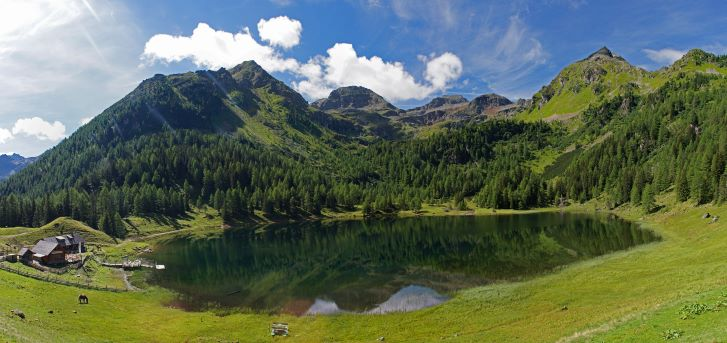
\includegraphics{fotolia-small.jpg}
\caption{Norway Spruce and Larch Forest in Austrian Alps,
\url{https://ec.europa.eu/jrc/en/research-topic/forestry/qr-tree-project/norway-spruce}}
\end{figure}

The data used in this example are derived from the R package
\emph{Functions and Datasets for ``Forest Analytics with R''}.

According to the documentation, the source of these data are: ``von
Guttenberg's Norway spruce (Picea abies {[}L.{]} Karst) tree measurement
data.''

The documentation goes on to further note that:

\begin{quote}
``The data are measures from 107 trees. The trees were selected as being
of average size from healthy and well stocked stands in the Alps.''
\end{quote}

\hypertarget{import-the-data}{%
\section{Import The Data 🌲}\label{import-the-data}}

\begin{verbatim}
## # A tibble: 1,200 x 9
##         site  location  tree age_base height dbh_cm volume age_bh   tree_ID
##    <dbl+lbl> <dbl+lbl> <dbl>    <dbl>  <dbl>  <dbl>  <dbl>  <dbl> <dbl+lbl>
##  1     1 [1]     1 [1]     1       20    4.2    4.6      5   9.67   1 [1.1]
##  2     1 [1]     1 [1]     1       30    9.3   10.2     38  19.7    1 [1.1]
##  3     1 [1]     1 [1]     1       40   14.9   14.9    123  29.7    1 [1.1]
##  4     1 [1]     1 [1]     1       50   19.7   18.3    263  39.7    1 [1.1]
##  5     1 [1]     1 [1]     1       60   23     20.7    400  49.7    1 [1.1]
##  6     1 [1]     1 [1]     1       70   25.8   22.6    555  59.7    1 [1.1]
##  7     1 [1]     1 [1]     1       80   27.4   24.1    688  69.7    1 [1.1]
##  8     1 [1]     1 [1]     1       90   28.8   25.5    820  79.7    1 [1.1]
##  9     1 [1]     1 [1]     1      100   30     26.5    928  89.7    1 [1.1]
## 10     1 [1]     1 [1]     1      110   30.9   27.3   1023  99.7    1 [1.1]
## # ... with 1,190 more rows
\end{verbatim}

\hypertarget{variables}{%
\section{Variables 🌲}\label{variables}}

\texttt{site} Growth \emph{quality} class of the tree's habitat. 5
levels.

\texttt{location} Distinguishes tree \emph{location}. 7 levels.

\texttt{tree} An identifier for the tree within location.

\texttt{age.base} The tree age taken at ground level.

\texttt{height} Tree height, m.

\texttt{dbh.cm} Tree diameter, cm.

\texttt{volume} Tree volume.

\texttt{age.bh} Tree age taken at 1.3 m.

\texttt{tree.ID} A factor uniquely identifying the tree.

\hypertarget{a-basic-multilevel-model}{%
\section{A Basic Multilevel Model}\label{a-basic-multilevel-model}}

\[\text{height}_{it} = \beta_0 + \beta \text{age_base} + \beta \text{site} + u_{0\text{ tree.ID}} + e_{it}\]

\end{document}
